\chapter{Creating a Repository (Stratum~0)}
\label{sct:createrepo}

% Introduction
% Components
% Installation / Requirements
% Cvmfs server and cvmfs swissknife

\cvmfs\ is a file system with a single source of (new) data.
This single source, the repository \emph{Stratum 0}, is maintained by a dedicated \emph{release manager machine} or \emph{installation box}.
A read-writable copy of the repository is accessible on the release manager machine.
The \cvmfs\ server tool kit is used to \emph{publish} the current state of the repository on the release manager machine.
Publishing is an atomic operation.

All data stored in \cvmfs\ have to be converted into a \cvmfs\ \emph{repository} during the process of publishing.
The \cvmfs\ repository is a form of content-addressable storage.
Conversion includes creating the file catalog(s), compressing new and updated files and calculating content hashes.
Storing the data in a content-addressable format results in automatic file de-duplication.
It furthermore simplifies data verification and it allows for file system snapshots.

In order to provide a writable \cvmfs\ repository, \cvmfs\ uses a union file system that combines a read-only \cvmfs\ mount point with a writable scratch area~\cite{unionfs04,aufs}.
Figure~\ref{fig:installwebserver} outlines the process of publishing a repository.

\pagebreak

\section{\cvmfs\ Server Quick-Start Guide}
\label{sct:quickstart}

\subsection{System Requirements}
\begin{itemize}
\item Apache HTTP server \emph{OR} S3 compatible storage service
\item AUFS union file system in the kernel
\item Officially supported platforms
\begin{itemize}
    \item Scientific Linux 5 (64 bit)
    \item Scientific Linux 6 (64 bit - with custom AUFS enabled kernel - Appendix~\ref{apx:rpms})
    \item Ubuntu 13.10 and above (64 bit - with installed AUFS kernel module)
\end{itemize}
\end{itemize}

\subsection{Installation}
\begin{enumerate}
\item Install \texttt{cvmfs} and \texttt{cvmfs-server} packages
\item Ensure enough disk space in \texttt{/var/spool/cvmfs} (\textgreater 50GiB)
\item For local storage: Ensure enough disk space in \texttt{/srv/cvmfs}
\item Create a repository with \texttt{cvmfs\_server mkfs} (See Section~\ref{sct:repocreation})
\end{enumerate}

\subsection{Content Publishing}
\begin{enumerate}
\item \texttt{cvmfs\_server transaction <repository name>}
\item Install content into \texttt{/cvmfs/<repository name>}
\item Create nested catalogs at proper locations
\begin{itemize}
    \item Create \texttt{.cvmfscatalog} files (See Section~\ref{sct:nestedcatalogs}) or
    \item Consider using a \texttt{.cvmfsdirtab} file (See Section~\ref{sct:dirtab})
\end{itemize}
\item \texttt{cvmfs\_server publish <repository name>}
\end{enumerate}

\subsection{Backup Policy}
\begin{itemize}
\item Create backups of signing key files in \texttt{/etc/cvmfs/keys}
\item Entire repository content
\begin{itemize}
   \item For local storage: \texttt{/srv/cvmfs}
   \item Stratum~1s can serve as last-ressort backup of repository content
\end{itemize}
\end{itemize}

\pagebreak

\section{Publishing a new Repository Revision}
\label{sct:repoupdate}

\begin{figure}[h]
	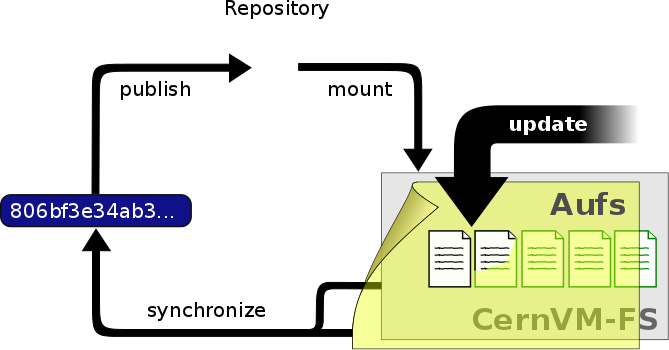
\includegraphics[width=\textwidth]{figures/update_process.png}
	\caption{Updating a mounted \cvmfs\ repository by overlaying it with a copy-on-write \aufs\ volume.
		Any changes will be accumulated in a writable volume (yellow) and can be synchronized into the \cvmfs\ repository afterwards.
		The file catalog contains the directory structure as well as file metadata, symbolic links, and secure hash keys of regular files.
		Regular files are compressed and renamed to their cryptographic content hash before copied into the data store.}
	\label{fig:installwebserver}
\end{figure}

Since the repositories may contain many file system objects\footnote{For ATLAS, for example, ``many'' means order of $10^7$ file system objects (\ie number of regular files, symbolic links, and directories).}, we cannot afford to generate an entire repository from scratch for every update.
Instead, we add a writable file system layer on top of a mounted read-only \cvmfs\ repository using the union file system \aufs~\cite{aufs}.
This renders a read-only \cvmfs\ mount point writable to the user, while all performed changes are stored in a special writable scratch area managed by \aufs.
A similar approach is used by Linux Live Distributions that are shipped on read-only media, but allow \emph{virtual} editing of files where changes are stored on a RAM disk.

If a file in the \cvmfs\ repository gets changed, \aufs\ first copies it to the writable volume and applies any changes to this copy (copy-on-write semantics).
\aufs\ will put newly created files or directories in the writable volume as well.
Additionally it creates special hidden files (called \emph{white-outs}) to keep track of file deletions in the \cvmfs\ repository.

Eventually, all changes applied to the repository are stored in \aufs's scratch area and can be merged into the actual \cvmfs\ repository by a subsequent synchronization step.
Up until the actual synchronization step takes place, no changes are applied to the \cvmfs\ repository.
Therefore, any unsuccessful updates to a repository can be rolled back by simply clearing the writable file system layer of \aufs.

\section{Requirements for a new Repository}
\label{sct:newreporequirements}

In order to create a repository, the server and client part of \cvmfs\ must be installed on the release manager machine.
Furthermore your machine should provide an \aufs\ enabled Kernel as well as a running \texttt{Apache2} web server.
Currently we support Scientific Linux 6 and Ubuntu 12.04 distributions.
Please note, that Scientific Linux 6 \emph{does not} ship with an \aufs\ enabled kernel, therefore we provide a compatible patched kernel as RPMs (see Appendix~\ref{apx:rpms}).


\pagebreak
\section{Notable \cvmfs\ Server Locations and Files}
\label{sct:repoanatomy}
There are a number of possible customisations in the \cvmfs\ server installation.
The following table provides an overview of important configuration files and intrinsical paths together with some customisation hints.
\LTXtable{\textwidth}{figures/tabserveranatomy.tex}


\section{\cvmfs\ Repository Creation and Updating}
\label{sct:repocreateandupdate}
The \cvmfs\ server tool kit provides the \texttt{cvmfs\_server} utility in order to perform all operations related to repository creation, updating, deletion, replication and inspection.
Without any parameters it prints a short documentation of its commands.

\subsection{Repository Creation}
\label{sct:repocreation}

A new repository is created by \texttt{cvmfs\_server mkfs}:
\begin{verbatim}
  cvmfs_server mkfs my.repo.name
\end{verbatim}
The utility will ask for a user that should act as the owner of the repository and afterwards create all the infrastructure for the new \cvmfs\ repository.
Additionally it will create a reasonable default configuration and generate a new release manager certificate and software signing key.
The public key in \texttt{/etc/cvmfs/keys/my.repo.name.pub} needs to be distributed to all client machines.

The \texttt{cvmfs\_server} utility will use \texttt{/srv/cvmfs} as storage location by default.
In case a separate hard disk should be used, a partition can be mounted on /src/cvmfs or /srv/cvmfs can be symlinked to another location (see Section~\ref{sct:repoanatomy}).
Besides local storage it is possible to use an S3 compatible storage service as data backend (see Section~\ref{sct:s3storagesetup}).

Once created, the repository is mounted under \texttt{/cvmfs/my.repo.name} containing only a single file called \texttt{new\_repository}.
The next steps describe how to change the repository content.

\subsubsection{Repositories for Volatile Files}
Repositories can be flagged as containing \emph{volatile} files using the \texttt{-v} option:
\begin{verbatim}
  cvmfs_server mkfs -v my.repo.name
\end{verbatim}
When \cvmfs\ clients perform a cache cleanup, they treat files from volatile repositories with priority.
Such volatile repositories can be useful, for instance, for experiment conditions data.

\subsubsection{S3 Compatible Storage Systems}
\label{sct:s3storagesetup}

\cvmfs\ can store files directly to S3 compatible storage systems, such as \product{Amazon S3}, \product{Huawei UDS} and \product{OpenStack SWIFT}.
The S3 storage settings are given as parameters to \texttt{cvmfs\_server mkfs}:
\begin{verbatim}
  cvmfs_server mkfs -s /etc/cvmfs/.../mys3.conf \
    -w http://s3.amazonaws.com/mybucket my.repo.name
\end{verbatim}

The file ``mys3.conf'' contains the S3 settings (see Table~\ref{tbl:s3confparameters}).
The ``-w'' option is used define the S3 server URL, e.g. http://localhost:3128, which is used for accessing the repository's backend storage on S3.
Note that this URL can be different than the S3 server address that is used for uploads, e.g. if a proxy server is deployed in front of the server.
Note that the buckets need to exist before the repository is created.
In the example above, a single bucket \texttt{mybucket-1-1} needs to be created beforehand.

\LTXtable{\textwidth}{figures/tabs3confparameters.tex}

In addition, if the S3 backend is configured to use multiple accounts or buckets, a proxy server is needed to map HTTP requests to correct buckets.
This mapping is needed because \cvmfs\ does not support buckets but assumes that all files are stored in a flat namespace.
The recommendation is to use a \squid\ proxy server (version $\geq 3.1.10$).
The squid.conf can look like this:
\begin{verbatim}
http_access allow all
http_port 127.0.0.1:3128 intercept
cache_peer swift.cern.ch parent 80 0 no-query originserver
url_rewrite_program /usr/bin/s3_squid_rewrite.py
cache deny all
\end{verbatim}

The bucket mapping logic is implemented in s3\_squid\_rewrite.py file.
This python script needs to read requests from stdin and write mapped URLs to stdout, for instance:
\begin{verbatim}
in: http://localhost:3128/data/.cvmfswhitelist
out: http://swift.cern.ch/cernbucket-9-91/data/.cvmfswhitelist
\end{verbatim}

\subsection{Repository Update}
\label{sct:repoupdateprocedure}
Typically a repository publisher does the following steps in order to create a new revision of a repository:
\begin{enumerate}
	\item Run \texttt{cvmfs\_server transaction} to switch to a copy-on-write enabled \cvmfs\ volume
	\item Make the necessary changes to the repository, \eg add new directories, patch certain binaries, \dots
	\item Test the software installation
	\item Do one of the following:
	\begin{itemize}
		\item Run \texttt{cvmfs\_server publish} to finalize the new repository revision \emph{or}
		\item Run \texttt{cvmfs\_server abort} to clear all changes and start over again
	\end{itemize}
\end{enumerate}

\cvmfs\ supports having more than one repository on a single server machine.
In case of a multi-repository host, the target repository of a command needs to be given as a parameter when running the \texttt{cvmfs\_server} utility.
The \texttt{cvmfs\_server resign} command should run every 30 days to update the signatures of the repository.
Most \texttt{cvmfs\_server} commands allow for wildcards to do manipulations on more than one repository at once, \eg \texttt{cvmfs\_server migrate *.cern.ch} would migrate all present repositories ending with \texttt{.cern.ch}.

\subsection{Repository Import}
The \cvmfs\ 2.1 server tools support the import of a \cvmfs\ file storage together with its corresponding signing keychain.
With \texttt{cvmfs\_server import} both \cvmfs\ 2.0 and 2.1 compliant repository file storages can be imported.

\texttt{cvmfs\_server import} works similar to \texttt{cvmfs\_server mkfs} (see \ref{sct:repocreation}) except it uses the provided data storage instead of creating a fresh (and empty) storage.
In case of a \cvmfs\ 2.0 file storage \texttt{cvmfs\_server import} also takes care of the file catalog migration into the \cvmfs\ 2.1 schema.

\subsubsection{Legacy Repository Import}
We strongly recommend to install \cvmfs\ 2.1 on a fresh or at least a properly cleaned  machine without any traces of the \cvmfs\ 2.0 installation before installing \cvmfs\ 2.1 server tools.

The command \texttt{cvmfs\_server import} requires the full \cvmfs\ 2.0 data storage which is located at /srv/cvmfs by default as well as the repository's signing keys.
Since the \cvmfs\ 2.1 server backend supports multiple repositories in contrast to its 2.0 counterpart, we recommend to move the repository's data storage to /srv/cvmfs/<FQRN> upfront to avoid later inconsistencies.

The following steps describe the transformation of a repository from \cvmfs\ 2.0 into 2.1. As an example we are using a repository called \textbf{legacy.cern.ch}.
\begin{enumerate}
	\item Make sure that you have backups of both the repository's backend storage and its signing keys
	\item Install and test the \cvmfs\ 2.1 server tools on the machine that is going to be used as new Stratum 0 maintenance machine
	\item Place the repository's backend storage data in /srv/cvmfs/\textit{legacy.cern.ch} \\ (default storage location)
	\item Transfer the repository's signing keychain to the machine (f.e. to \textapprox/legacy\_keys/)
	\item Run \texttt{cvmfs\_server import} like this:
\begin{verbatim}
    cvmfs_server import
      -o <username of repo maintainer> \
      -k ~/legacy_keys \
      -l               \ # for 2.0.x file catalog migration
      -s               \ # for further repository statistics
      legacy.cern.ch
\end{verbatim}
    \item Check the imported repository with \texttt{cvmfs\_server check legacy.cern.ch} for integrity (see \ref{sct:checkintegrity})
\end{enumerate}


\subsection{Customizable Actions Using Server Hooks}
\label{sct:serverhooks}
The \texttt{cvmfs\_server} utility allows release managers to trigger custom actions before and after crucial repository manipulation steps. This can be useful for example for logging purposes, establishing backend storage connections automatically or other workflow triggers, depending on the application.

There are six designated server hooks that are potentially invoked during the repository update procedure described in Section \ref{sct:repoupdateprocedure}:
\begin{itemize}
	\item When running \texttt{cvmfs\_server transaction}:
	\begin{itemize}
		\item \emph{before} the given repository is transitioned into transaction mode
		\item \emph{after} the transition was successful
	\end{itemize}
	\item When running \texttt{cvmfs\_server publish}:
	\begin{itemize}
		\item \emph{before} the publish procedure for the given repository is started
		\item \emph{after} it was published and remounted successfully
	\end{itemize}
	\item When running \texttt{cvmfs\_server abort}:
	\begin{itemize}
		\item \emph{before} the unpublished changes will be erased for the given repository
		\item \emph{after} the repository was successfully reverted to the last published state
	\end{itemize}
\end{itemize}
All server hooks must be defined in a single shell script file called:
\begin{verbatim}
/etc/cvmfs/cvmfs_server_hooks.sh
\end{verbatim}
The \texttt{cvmfs\_server} utility will check the existence of this script and source it.
To subscribe to the described hooks one needs to define one or more of the following shell script functions:
\begin{itemize}
	\setlength{\itemsep}{1pt}
	\item \texttt{transaction\_before\_hook()}
	\item \texttt{transaction\_after\_hook()}
\end{itemize}
\begin{itemize}
	\item \texttt{publish\_before\_hook()}
	\item \texttt{publish\_after\_hook()}
\end{itemize}
\begin{itemize}
	\item \texttt{abort\_before\_hook()}
	\item \texttt{abort\_after\_hook()}
\end{itemize}
The defined functions get called at the specified positions in the repository update process and are provided with the fully qualified repository name as their only parameter~(\texttt{\$1}).
Undefined functions automatically default to a NO-OP.
An example script is located at \texttt{cvmfs/cvmfs\_server\_hooks.sh.demo} in the \cvmfs\ sources.


\section{Maintaining a CernVM-FS Repository}

\cvmfs\ is a versioning, snapshot-based file system.
Similar to versioning systems, changes to /cvmfs/\dots are temporary until they are committed (\texttt{cvmfs\_server publish}) or discarded (\texttt{cvmfs\_server abort}).
That allows you to test and verify changes, for instance to test a newly installed release before publishing it to clients.
Whenever changes are published (committed), a new file system snapshot of the current state is created.
These file system snapshots can be tagged with a name, which makes them \emph{named snapshots}.
A named snapshot is meant to stay in the file system.
One can rollback to named snapshots and it is possible, on the client side, to mount any of the named snapshots in lieu of the newest available snapshot.

Two named snapshots are managed automatically by \cvmfs, \texttt{trunk} and \texttt{trunk-previous}.
This allows for easy unpublishing of a mistake, by rolling back to the \texttt{trunk-previous} tag.

\subsection{Integrity Check}
\label{sct:checkintegrity}
\cvmfs\ provides an integrity checker for repositories.
It is invoked by
\begin{verbatim}
cvmfs_server check
\end{verbatim}

The integrity checker verifies the sanity of file catalogs and verifies that referenced data chunks are present.
Ideally, the integrity checker is used after every publish operation.
Where this is not affordable due to the size of the repositories, the integrity checker should run regularly.

Optionally \texttt{cvmfs\_server check} can also verify the data integrity (command line flag \texttt{-i}) of each data object in the repository.
This is a time consuming process and we recommend it only for diagnostic purposes.


\subsection{Named Snapshots}
\label{sct:namedsnapshots}

Named snapshots or \emph{tags} are an easy way to organise checkpoints in the file system history.
\cvmfs\ clients can explicitly mount a repository at a specific named snapshot to expose the file system content published with this tag.
It also allows for rollbacks to previously created and tagged file system revisions.
Tag names need to be unique for each repository and are not allowed to contain spaces or spacial characters.
Besides the actual tag's name they can also contain a free descriptive text and store a creation timestamp.

Named snapshots are best to use for larger modifications to the repository, for instance when a new major software release is installed.
Named snapshots provide the ability to easily undo modifications and to preserve the state of the file system for the future.
Nevertheless, named snapshots should not be used excessively.
Less than 50 named snapshots are a good number of named snapshots in many cases.

By default, new repositories will automatically create a generic tag if no explicit tag is given during publish.
The automatic tagging can be turned off using the -g option during repository creation or by setting \texttt{CVMFS\_AUTO\_TAG=false} in the /etc/cvmfs/repositories.d/\$repository/server.conf file.

\subsubsection{Creating a Named Snapshot}
Tags can be added while publishing a new file system revision.
To do so, the -a and -m options for \texttt{cvmfs\_server publish} are used.
The following command publishes a \cvmfs\ revision with a new revision that is tagged as ``release-1.0'':
\begin{verbatim}
cvmfs_server transaction
# Changes
cvmfs_server publish -a release-1.0 -m "first stable release"
\end{verbatim}

\subsubsection{Managing Existing Named Snapshots}
Management of existing tags is done by using the \texttt{cvmfs\_server tag} command.
Without any command line parameters, it will print all currently available named snapshots.
Snapshots can be inspected (\texttt{-i <tag name>}), removed (\texttt{-r <tag name>}) or created (\texttt{-a <tag name> -m <tag description> -h <catalog root hash>}).
Furthermore machine readable modes for both listing (\texttt{-l -x}) as well as inspection (\texttt{-i <tag name> -x}) is available.

\subsubsection{Rollbacks}
A repository can be rolled back to any of the named snapshots.
Rolling back is achieved through the command \texttt{cvmfs\_server rollback -t release-1.0}
A rollback is, like restoring from backups, not something one would do often.
Use caution, a rollback is irreversible.

\subsection{Manage Nested Catalogs}
\label{sct:nestedcatalogs}

\cvmfs\ stores meta-data (path names, file sizes, \dots) in file catalogs.
When a client accesses a repository, it has to download the file catalog first and then it downloads the files as they are opened.
A single file catalog for an entire repository can quickly become large and impractical.
Also, clients typically do not need all of the repository's meta-data at the same time.
For instance, clients using software release 1.0 do not need to know about the contents of software release 2.0.

With nested catalogs, \cvmfs\ has a mechanism to partition the directory tree of a repository into many catalogs.
Repository maintainers are responsible for sensible cutting of the directory trees into nested catalogs.
They can do so by creating and removing magic files named \texttt{.cvmfscatalog}.

For example, in order to create a nested catalog for software release 1.0 in the hypothetical repository experiment.cern.ch, one would invoke
\begin{verbatim}
cvmfs_server transaction
touch /cvmfs/experiment.cern.ch/software/1.0/.cvmfscatalog
cvmfs_server publish
\end{verbatim}

In order to merge a nested catalog with its parent catalog, the corresponding \texttt{.cvmfscatalog} file needs to be removed.
Nested catalogs can be nested on arbitrary many levels.

\subsection{Recommendations for Nested Catalogs}
\label{sct:nestedcatalogrecommendations}
Nested catalogs should be created having in mind which files and directories are accessed together.
This is typically the case for software releases, but can be also on the directory level that separates platforms.
For instance, for a directory layout like
\begin{verbatim}
/cvmfs/experiment.cern.ch
  |- /software
  |    |- /i686
  |    |    |- 1.0
  |    |    |- 2.0
  |    `    |- common
  |    |- /x86_64
  |    |    |- 1.0
  |    `    |- common
  |- /grid-certificates
  |- /scripts
\end{verbatim}
it makes sense to have nested catalogs at
\begin{verbatim}
/cvmfs/experiment.cern.ch/software/i686
/cvmfs/experiment.cern.ch/software/x86_64
/cvmfs/experiment.cern.ch/software/i686/1.0
/cvmfs/experiment.cern.ch/software/i686/2.0
/cvmfs/experiment.cern.ch/software/x86_64/1.0
\end{verbatim}

A nested catalog at the top level of each software package release is generally the best approach because once package releases are installed they tend to never change, which reduces churn and garbage generated in the repository from old catalogs that have changed.
In addition, each run only tends to access one version of any package so having a separate catalog per version avoids loading catalog information that will not be used.
A nested catalog at the top level of each platform may make sense if there is a significant number of platform-specific files that aren't included in other catalogs.

It could also make sense to have a nested catalog under grid-certificates, if the certificates are updated much more frequently than the other directories.
It would not make sense to create a nested catalog under /cvmfs/experiment.cern.ch/software/i686/common, because this directory needs to be accessed anyway whenever its parent directory is needed.
As a rule of thumb, a single file catalog should contain more than 1000 files and directories but not contain more than $\approx$200\,000 files.
Section~\ref{sct:inspectnestedcatalogs} describes how to find catalogs that do not satisfy this recommendation.

Restructuring the repository's directory tree is an expensive operation in CernVM-FS.
Moreover, it can easily break client applications when they switch to a restructured file system snapshot.
Therefore, the software directory tree layout should be relatively stable before filling the CernVM-FS repository.

\subsection{Managing Nested Catalogs with \texttt{.cvmfsdirtab}}
\label{sct:dirtab}
Rather than managing \texttt{.cvmfscatalog} files by hand, a repository administrator may create a file called \texttt{.cvmfsdirtab}, in the top directory of the repository, which contains a list of paths relative to the top of the repository where \texttt{.cvmfscatalog} files will be created.
Those paths may contain shell wildcards such as asterisk (\texttt{*}) and question mark (\texttt{?}).
This is useful for specifying patterns for creating nested catalogs as new files are installed.
A very good use of the patterns is to identify directories where software releases will be installed.

In addition, lines in \texttt{.cvmfsdirtab} that begin with an exclamation point (\texttt{!}) are shell patterns that will be excluded from those matched by lines without an exclamation point.
For example a \texttt{.cvmfsdirtab} might contain these lines for the repository of the previous subsection:
\begin{verbatim}
/software/*
/software/*/*
! */common
/grid-certificates
\end{verbatim}
This will create nested catalogs at
\begin{verbatim}
/cvmfs/experiment.cern.ch/software/i686
/cvmfs/experiment.cern.ch/software/i686/1.0
/cvmfs/experiment.cern.ch/software/i686/2.0
/cvmfs/experiment.cern.ch/software/x86_64
/cvmfs/experiment.cern.ch/software/x86_64/1.0
/cvmfs/experiment.cern.ch/grid-certificates
\end{verbatim}
Note that unlike the regular lines that add catalogs, asterisks in the exclamation point exclusion lines can span the slashes separating directory levels.

\subsection{Inspecting Nested Catalog Structure}
\label{sct:inspectnestedcatalogs}
The following command visualizes the current nested file catalog layout of a repository.

\begin{verbatim}
cvmfs_server list-catalogs
\end{verbatim}

Additionally this command allows to spot degenerated nested catalogs.
As stated in Section~\ref{sct:nestedcatalogrecommendations} the recommended maximal file entry count of a single catalog should not exceed $\approx$200\,000.
One can use the switch \texttt{list-catalogs -e} to inspect the current nested catalog entry counts in the repository.
Furthermore \texttt{list-catalgos -s} will print the file sizes of the catalogs in bytes.

\subsection{Migrate File Catalogs}
In rare cases the further development of \cvmfs\ makes it necessary to change the internal structure of file catalogs.
Updating the \cvmfs\ installation on a Stratum 0 machine might require a migration of the file catalogs.

It is recommended that \texttt{cvmfs\_server list} is issued after any \cvmfs\ update to review if any of the maintained repositories need a migration.
Outdated repositories will be marked as ``INCOMPATIBLE'' and \texttt{cvmfs\_server} refuses all actions on these repositories until the file catalogs have been updated.

In order to run a file catalog migration use \texttt{cvmfs\_server migrate} for each of the outdated repositories.
This will essentially create a new repository revision that contains the exact same  file structure as the current revision.
However, all file catalogs will be recreated from scratch using the updated internal structure.
Note that historic file catalogs of all previous repository revisions stay untouched and are not migrated.

After \texttt{cvmfs\_server migrate} has successfully updated all file catalogs repository maintenance can continue as usual.



\section{Repository Garbage Collection}
\label{sct:garbagecollection}
Since \cvmfs\ is a versioning file system it is following an insert-only policy regarding its backend storage.
When files are deleted from a \cvmfs\ repository, they are not automatically deleted from the underlying storage.
Therefore legacy revisions stay intact and usable forever (cf. Section~\ref{sct:namedsnapshots}) at the expense of an ever-growing storage volume both on the Stratum~0 and the Stratum~1s.

For this reason, applications that frequently install files into a repository and delete older ones -- for example the output from nightly software builds -- might quickly fill up the repository's backend storage.
Furthermore these applications might actually never make use of the aforementioned long-term revision preservation rendering most of the stored objects ``garbage''.

\cvmfs\ supports garbage-collected repositories that automatically remove unreferenced data objects and free storage space.
This feature needs to be enabled on the Stratum~0 and automatically scans the repository's catalog structure for unreferenced objects both on the Stratum~0 and the Stratum~1 installations on every publish respectively snapshot operation.

\subsection{Garbage Sweeping Policy}
The garbage collector of \cvmfs\ is using a mark-and-sweep algorithm to detect unused files in the internal catalog graph.
%For this it classifies all available repository revisions into \emph{preserved} and \emph{condemned} revisions.
%All stored objects that are referenced only in the condemned but \emph{not} in the preserved revisions -- including catalog files -- are considered garbage and will be removed.
%
Revisions that are referenced by named snapshots (cf. Section~\ref{sct:namedsnapshots}) or that are recent enough are preserved while all other revisions are condemned to be removed.
By default this time-based threshold is \emph{three days} but can be changed using the configuration variable \texttt{CVMFS\_AUTO\_GC\_TIMESPAN} both on Stratum~0 and Stratum~1.
The value of this variable is expected to be parseable by the \texttt{date} command, for example \texttt{3 days ago} or \texttt{1 week ago}.

\subsection{Enabling Garbage Collection}
\label{sct:enablegc}

\subsubsection{Creating a Garbage Collectable Repository}
Repositories can be created as \emph{garbage-collectable} from the start by adding \texttt{-z} to the \texttt{cvmfs\_server mkfs} command (cf. Section~\ref{sct:repocreation}).
It is generally recommended to also add \texttt{-g} to switch off automatic tagging in a garbage collectable repository.

\subsubsection{Enabling Garbage Collection on an Existing Repository (Stratum 0)}
Existing repositories can be reconfigured to be garbage collectable by adding\\ \texttt{CVMFS\_GARBAGE\_COLLECTION=true} and \texttt{CVMFS\_AUTO\_GC=true} to the \texttt{server.conf} of the repository.
Furthermore it is recommended to switch off automatic tagging by setting \texttt{CVMFS\_AUTO\_TAG=false} for a garbage collectable repository.
The garbage collection will be enabled with the next published transaction.

\subsubsection{Enabling Garbage Collection on an Existing Replication (Stratum 1)}
In order to use automatic garbage collection on a stratum 1 replica \texttt{CVMFS\_AUTO\_GC=true} needs to be added in the \texttt{server.conf} file of the stratum 1 installation.
This will only work if the upstream stratum 0 repository has garbage collection enabled.

\section{Limitations on Repository Content}
Because \cvmfs\ provides what appears to be a POSIX filesystem to clients, it is easy to think that it is a general purpose filesystem and that it will work well with all kinds of files.
That is not the case, however, because \cvmfs\ is optimized for particular types of files and usage.
This section contains guidelines for limitations on the content of repositories for best operation.

\subsection{Data files}
First and foremost, \cvmfs\ is designed to distribute executable code that is shared between a large number of jobs that run together at grid sites, clouds, or clusters.
Worker node cache sizes and web proxy bandwidth are generally engineered to accommodate that application.
The total amount read per job is expected to be roughly limited by the amount of RAM per job slot.
The same files are also expected to be read from the worker node cache multiple times for the same type of job, and read from a caching web proxy by multiple worker nodes.

If there are data files distributed by \cvmfs\ that follow similar access patterns and size limits as executable code, it will probably work fine.
In addition, if there are files that are larger but read slowly throughout long jobs, as opposed to all at once at the beginning, that can also work well if the same files are read by many jobs.
That is because web proxies have to be engineered for handling bursts at the beginning of jobs and so they tend to be lightly loaded a majority of the time.

In general, a good rule of thumb is to calculate the maximum rate at which jobs typically start and limit the amount of data that might be read from a web proxy to \SI{100}{\mega\byte\per\second} per thousand jobs, assuming a reasonable amount of overlap of jobs onto the same worker nodes.
Also, limit the amount of data that will be put into any one worker node cache to \SI{5}{\giga\byte}.
Of course, if you have a special arrangement with particular sites to have large caches and bandwidths available, these limits can be made higher at those sites.
Web proxies may also need to be engineered with faster disks if the data causes their cache hit ratios to be reduced.

Also, keep in mind that the total amount of data distributed is not unlimited.
The files are stored and distributed compressed, and files with the same content stored in multiple places in the same repository are collapsed to the same file in storage, but the storage space is used not only on the original repository server, it is also replicated onto multiple Stratum 1 servers.
Generally if only executable code is distributed, there is no problem with the space taken on Stratum 1s, but if many large data files are distributed they may exceed the Stratum 1
storage capacity.
Data files also tend to not compress as well, and that is especially the case of course if they are already compressed before installation.

\subsection{Tarballs, zip files, and other archive files}
If the contents of a tarball, zip file, or some other type of archive file is desired to be distributed by \cvmfs, it is usually better to first unpack it into its separate pieces first.
This is because it allows better sharing of content between multiple releases of the file;
some pieces inside the archive file might change and other pieces might not in the next release, and pieces that don't change will be stored as the same file in the repository.
\cvmfs\ will compress the content of the individual pieces, so even if there's no sharing between releases it shouldn't take much more space.

\subsection{File permissions}
Care should be taken to make all the files in a repository readable by ``other''.
This is because permissions on files in the original repository are generally the same as those seen by end clients, except the files are owned by the ``cvmfs'' user and group.
The write permissions are ignored by the client since it is a read-only filesystem.
However, unless the client has set
\begin{verbatim}
  CVMFS_CHECK_PERMISSIONS=no
\end{verbatim}
(and most do not), unprivileged users will not be able to read files unless they are readable by ``other'' and all their parent directories have at least ``execute'' permissions.
It makes little sense to publish files in \cvmfs\ if they won't be able to be read by anyone.

\subsection{Hardlinks}
By default \cvmfs\ does not allow hardlinks of a file to be in different directories.
If there might be any such hardlinks in a repository, set the option
\begin{verbatim}
    CVMFS_IGNORE_XDIR_HARDLINKS=true
\end{verbatim}
in the repository's \texttt{server.conf}.
The file will not appear to be hardlinked to the client, but it will still be stored as only one file in the repository just like any other files that have identical content.
Note that if, in a subsequent publish operation, only one of these cross-directory hardlinks gets changed, the other hardlinks remain unchanged (the hardlink got ``broken'').
